\part{System design}

In this chapter, design of the radio link and component selection are described. During the design process, multiple iteration of component selection, validation and link budget calculation were made, this chapter describes the final result of the design.

\chapter{Communication sessions}
PW-Sat2 was designed to be deployed on \SI{600}{\kilo\meter}, Sun-synchronous, polar orbit. Due to the Earts rotation, ground station coverage is bounded, and communication with the satellite is limited to communication session during satellite overpass.

Simulations performed using Gpredict software \cite{gpredict_website} shown that communication sessions will happen \si{5}-\si{6} times per day, \si{5}-\SI{10}{\minute} each. This summarizes to the total communication time to average \SI{30}{\minute} per day. Typical radio coverage of the satellite is shown in the figure \ref{gpredict_pass}.

\begin{figure}[H]
    \centering
    \includegraphics[width=0.8\paperwidth]{img/3/gpredict_pass.png}
    \caption{PW-Sat2 pass in Gpredict software.}
    \label{gpredict_pass}
\end{figure}


\chapter{Communication design requirements}
PW-Sat2 have couple of data sources to be sent to the ground:
\begin{itemize}
    \item housekeeping telemetry (satellite health information, such as temperatures, bus and solar panel voltages and currents, subsystem status etc. Telemetry is \SI{230}{\byte} frame and should be transmitted every \SI{1}{\minute} (average \SI{30}{\bps}),
    \item archival housekeeping telemetry (gathered during orbit, when no ground station is in range), telemetry should be downloaded in \SI{5}{\minute} step from the whole operational time, which sums up to \SI{64}{\kilo\byte} per day (average \SI{300}{\bps}),
    \item experiment data, which are started by the operator from the ground and each of them is planned to run once a week (Sun Sensor -  \SI{32}{\kilo\byte}, RadFET - \SI{4}{\kilo\byte}, Cameras (10 photos) - \SI{300}{\kilo\byte}) - it sums up to \SI{336}{\kilo\byte} per week, average of \SI{220}{\bps},
    \item Sail deployment procedure, which transmits experiment data on-line (during the experiment). Estimated data to be transmitted (sail deployment indicator, photos and gyroscopes) is about \SI{1}{\kbps}.
\end{itemize}

Data throughput requirement for PW-Sat2 mission sums up to about \SI{1}{\kbps}.

\chapter{Frequency band selection}
The most common radio bands used in CubeSat designs are VHF, UHF and S-band. S-band is usually used when high data rate (~\SI{10}{\Mbps}) are necessary. Typical designs for low-rate data link are full-duplex combo or simplex VHF/UHF radio.

PW-Sat1 \cite{pwsat1_website_ska} used full-duplex VHF-downlink and UHF-uplink radio. During its mission, operation team was reporting uplink stability issues, which was caused by very low Signal to Noise ratio on the satellite. The design team narrowed down the issue to very high level of interference in the UHF band on the orbit, which probably is caused by the high power signal sources on the ground, such as radars.

The selected bands for PW-Sat2 operation were either simplex VHF or full-duplex: VHF-up, UHF-down.


\chapter{Space segment}
Space segment is a part of the satellite communication system that resides on the satellite itself. It is divided into two main parts: communication subsystem (COMM) and antennas (ANTs) connected with two coaxial cables.

Space segment is critical in system operation and reliability - there is no possibility to carry out any repairs, perform maintenance or adjustment once on orbit. It is exposed to the space environment - wide temperature range, thermal cycling, cosmic radiation and vacuum.

Because of the mentioned requirements it was decided to choose commercially available and flight-proven CubeSat components to increase the overall reliability of the system.

\section{Communication subsystem}
CubeSat design specification \cite{cubesat_spec}, with which PW-Sat2 is compliant, defines common PC/104 connector, which is the main data bus for all satellite subsystems. On the connector, two \iic and two CAN buses are defined and most of the components are compatible to each other. However, due to the lack of CAN interface on On-Board Computer (CubeComputer from CubeSpace \cite{cubespace_website}) radio should use \iic communication bus.

When the subsystem was ordered (in year \si{2014}), the choice of available products was very limited, and the only radio which was compliant with above mentioned requirements was \texttt{ISIS VHF uplink/UHF downlink Full Duplex Transceiver}. Its view and block diagram is shown in the figure \ref{ISIS_TRXvU}

\begin{figure*}
   \centering
\begin{tabular}{cc}
        \includegraphics[width=0.3\paperwidth]{img/3/ISIS-radio-UHF-VHF-min.png}
    & 
        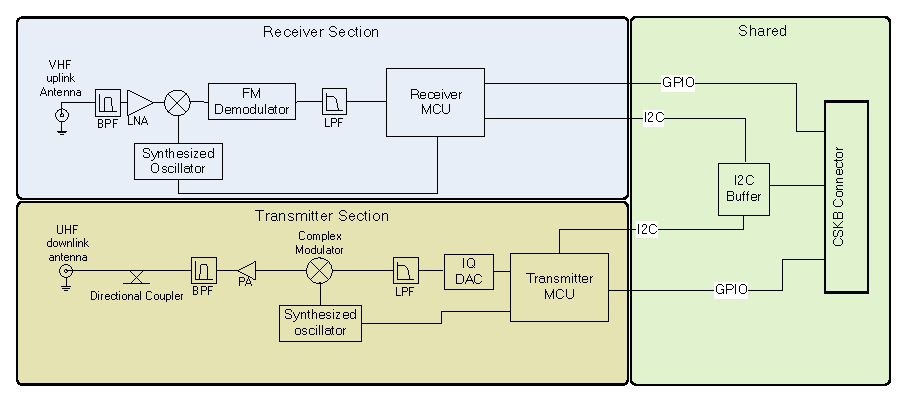
\includegraphics[width=0.4\paperwidth]{img/3/ISIS_TRXvU_block_diagram.eps}
\end{tabular}
\label{ISIS_TRXvU}
\caption{ISIS VHF uplink/UHF downlink Full Duplex Transceiver. Source: \cite{isis_trxvu}}
\end{figure*}

Basic characteristics: \\
\begin{tabular}{c|c}
     \textbf{downlink} & \textbf{uplink} \\ \hline
     \multicolumn{2}{c}{dual-\iic communication standard} \\
     \multicolumn{2}{c}{AX.25 frame format} \\
     \si{430}-\SI{450}{\MHz} frequency range & \si{140}-\SI{150}{\MHz} frequency range \\
     \SI{0.5}{\watt} downlink power & \SI{-98}{\dBm} sensitivity for \si{10^-5}~BER \\
     \si{1.2} - \SI{9.6}{\kilo\bit / \second} bitrate & \SI{1.2}{\kilo\bit / \second} bitrate \\ 
     BPSK modulation with G3RUH scrambling & FM-modulated AFSK \\ 
\end{tabular}


\section{Antennas}
Because of the selected radio system, two antennas has to be installed - one for uplink (VHF) and one for downlink (UHF). Antennas should be omnidirectional, as PW-Sat2 does not have an nadir-pointing capability and random tumbling during operation is assumed.

Self-made dipole antenna was considered at the design stage, but due to mechanical and time constraints, satellite antenna was decided to be bought as well. Innovative Solutions In Space company sells antenna with with the transceiver as CubeSat communication Kit \texttt{CubeSat dipole antenna system}. Both elements are compatibile and the whole system (transceiver + antenna) is tuned for specific communication frequency and mounting option.

This system is deployable by the command from the on-board computer. Thermal knife (resistor) is heated up and thermal link is burnt, resulting is antenna deploy by the spring action. Antenna is shown in the figure \ref{ISIS_antenna}.

\begin{figure*}
   \centering
\begin{tabular}{cc}
        \includegraphics[width=0.3\paperwidth]{img/3/isis_antenna_stowed.jpg}
    & 
        \includegraphics[width=0.45\paperwidth]{img/3/CubeSat-antenna-dipole-configuration.png}    
\end{tabular}
\label{ISIS_antenna}
\caption{ISIS CubeSat dipole antenna system in stowed and deployed position. Source: \cite{isis_dipole_antenna}}
\end{figure*}


% \subsection{Deployable elements influence on the antenna pattern}
% TODO

% On-board PW-Sat2 are two main deployables: solar panels and deorbitation sail.

% During design stage, influence of the solar panels was discussed with antenna manufacturer - the outcome was to place longed dipoles (VHF) along the solar panels, and shorter ones orthogonally to it, as shown in the figure \ref{???}

% % TODO: zdjęcie z otwartymi panelami i antenami

% The influence of the deorbit sail was also simulated during Critical Design stage.

% Deorbitation sail is made by very thin (\SI{5}{\micro\meter}) mylar foil with aluminium coating. Using % TODO
% simulation tool, it was shown that the sail will increase directivity of the cubesat antennas, acting as a reflector.
% % TODO: jakieś zdjęcie z symulacji, wynik o ile dB się pogorszyło


\chapter{Communication link parameters}
Selected satellite radio module imposes the modulation and data packets used in the communication. This section briefly describes used modulations, frame formats and implications to the ground segment of the system.

\section{Downlink modulation}
Downlink signal is modulated using Binary Phase Shift Keying (BPSK). The data rate can be changed dynamically by the spacecraft On-Board Computer, in range \si{1.2} - \SI{9.6}{\kbps}, allowing to improve the link quality when necessary. Baseband signal is also filtered using Raised Root Cosine filter, to reduce side lobes power. Signal bandwidth varies between \SI{2.4}{\kHz} (for \SI{1.2}{\kbps}) and \SI{19.2}{\kHz} (for \SI{9.6}{\kbps}).

% TODO: rysunek BPSK

\section{Uplink}
Uplink modulation is two-staged: first, data is modulated using Audio Frequency Shift Keying (chaning 0s and 1s to wave of frequencies, in order, \SI{1200}{\hertz} and \SI{2200}{\hertz}), later to be Frequency Modulated to the RF carrier (with frequency deviation of $\pm\SI{5}{\kilo\hertz}$).

% TODO: schemat modulatora

\section{Frame format}
Physical layer data format is reduced-functionality AX.25 packet \cite{AX25_standard}. Only connectionless transmission mode and UI frames are supported. Packet framing is the same as in SwissCube CubeSat \cite{SwissCube_AX25}.

Basic frame format is shown in the table \ref{AX25_frame}. All the fields except flags are bit-stuffed to ensure that the \textit{Flag} field does not appear in the data: if there are six '1' bits to be send, transmitter inserts '0' bit before the last one. Adressing in this system in inherent, but unused - this is point-to-point connection, therefore adresses are fixed. Frame-Check Sequence is a CRC (CITT standard) of the whole frame (without \textit{Flags}). \textit{Information Field} is variable-length, between \si{4} and \SI{256}{\byte} length is the place for the actual data transmitted by the On-Board Computer.

\begin{table}
\small
\centering
\caption{AX.25 frame format}
\label{AX25_frame}
\arrayrulecolor{black}
\begin{tabular}{l|c|c|c|c|c|c|c|c|} 
\hhline{~|-|----|-|-|-|}
\multirow{2}{*}{}                                                              & \multirow{2}{*}{Flag } & \multicolumn{4}{c|}{AX.25 Transfer Frame Header (128 bits)}                                                                                                                                                                                   & {\cellcolor[rgb]{0.753,0.753,0.753}}                                                                                                                  & \multirow{2}{*}{\begin{tabular}[c]{@{}c@{}}Frame-\\Check\\Sequence\end{tabular}} & \multirow{2}{*}{Flag}  \\ 
\hhline{~|~|-|-|-|-|>{\arrayrulecolor[rgb]{0.753,0.753,0.753}}->{\arrayrulecolor{black}}|~|~|}
                                                                               &                        & \begin{tabular}[c]{@{}c@{}}Destination\\Address\end{tabular} & \begin{tabular}[c]{@{}c@{}}Source\\Address\end{tabular} & \begin{tabular}[c]{@{}c@{}}Control\\Bits\end{tabular} & \begin{tabular}[c]{@{}c@{}}Protocol\\Identifier\end{tabular} & \multirow{-2}{*}{{\cellcolor[rgb]{0.753,0.753,0.753}}\begin{tabular}[c]{@{}>{\cellcolor[rgb]{0.753,0.753,0.753}}c@{}}Information\\Field\end{tabular}} &                                                                                  &                        \\ 
\hline
\multicolumn{1}{|c|}{\begin{tabular}[c]{@{}c@{}}Length\\{[}bits]\end{tabular}} & 8                      & 56                                                           & 56                                                      & 8                                                     & 8                                                            & {\cellcolor[rgb]{0.753,0.753,0.753}}32-2048                                                                                                           & 16                                                                               & 8                      \\ 
\hline
\multicolumn{1}{|c|}{Value}                                                    & 01111110               & PWSAT2-0                                                     & PWSAT2-0                                                & 00000011                                              & 11110000                                                     & {\cellcolor[rgb]{0.753,0.753,0.753}}                                                                                                                  & CRC-CITT                                                                         & 01111110               \\
\hline
\end{tabular}
\end{table}


Additionally, downlink data is scrambled using G3RUH scrambling polynomial to maximize randomness and ensure proper bit synchronization.

%% -------------------------------------------------------------------------------------------

\chapter{Ground station design}
Ground station design should complement the space segment, with large antenna gains and output power to allow the budget link to close. As the system is full-duplex, both uplink and downlink channels are separate and the design should allow to simultaneously operate transmit and receive. Block diagram of the designed ground station is shown in the figure \ref{gs_block_diagram}.
Due to the low sensitivity of the satellite receiver (\SI{-98}{\dBm}) uplink EIRP has to be very large, this is achieved by using high-power amplifier and antennas with high directional gain. For downlink, ground station has to compensate low transmit power of the satellite, by using high gain antennas and very sensitive receiver.

Ground station consists of not only the hardware but also software. Many parts of the system use Digital Signal Processing and Software-Defined Radio for data modulation/de-modulation, packet transmission etc. For the DSP tasks, GNUradio \cite{gnuradio} was selected and the tool for sampling-based signal processing.



\begin{figure}[H]
    \centering
    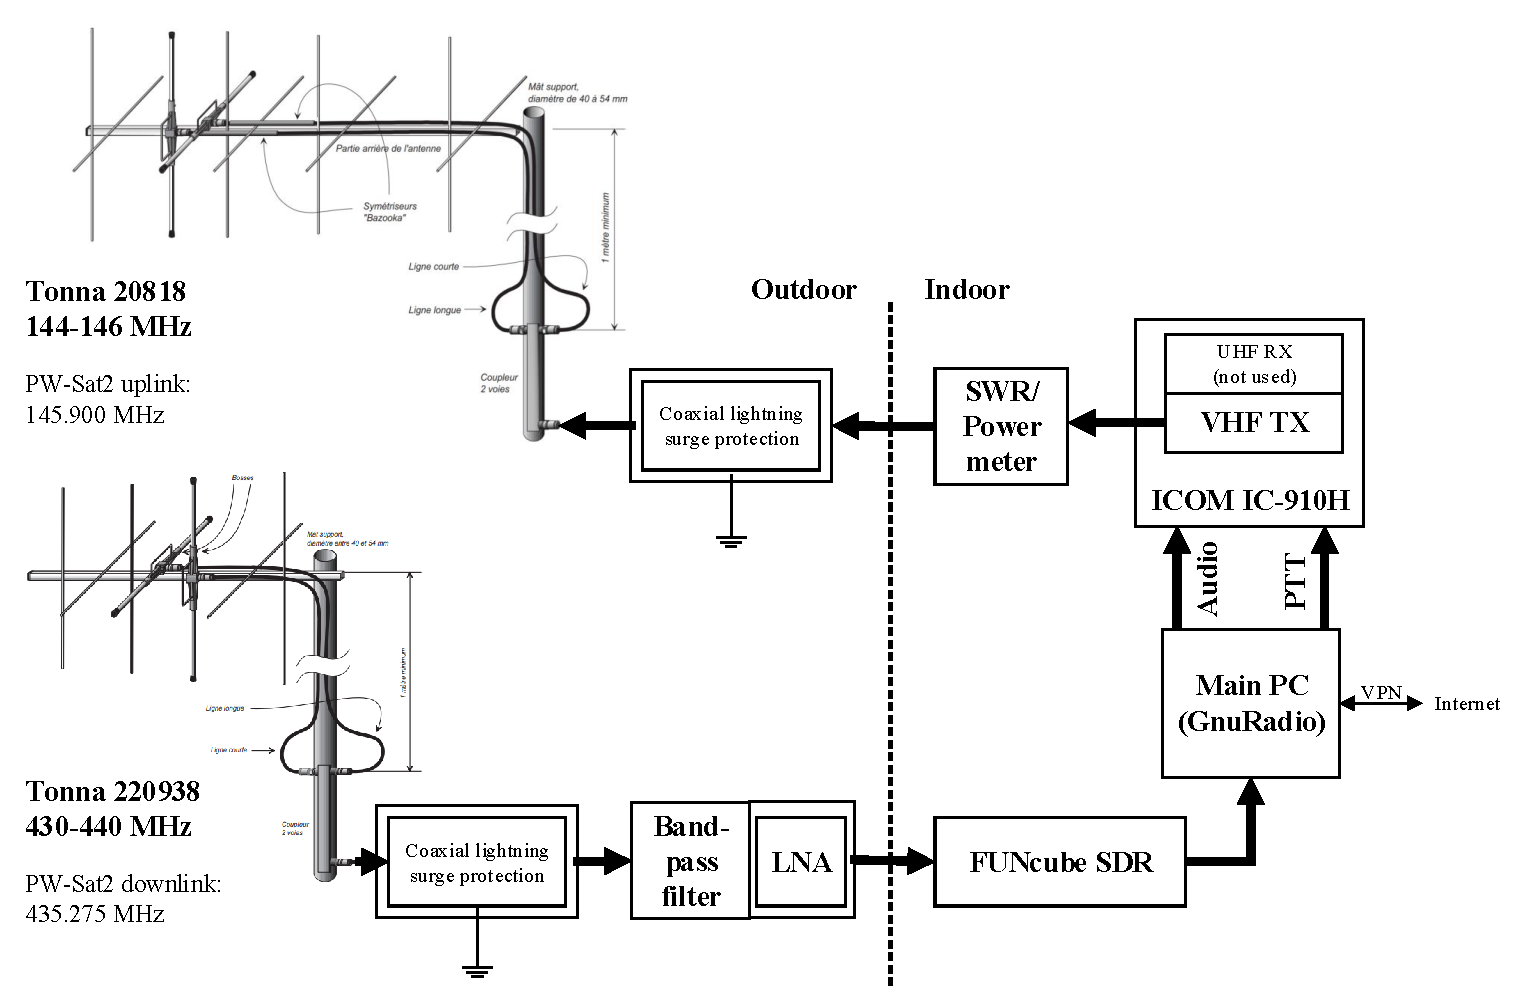
\includegraphics[width=0.8\paperwidth]{img/3/gs_block_diagram.eps}
    \caption{Ground station block diagram}
    \label{gs_block_diagram}
\end{figure}


\section{Antennas}
PW-Sat2 is transmitting radio signals with linear polarization, nevertheless ground station  polarization should be circular, due to the random tumbling of the satellite. This will reduce the gain of the antennas, but the signal strength will be constant regardless of the satellite rotation. Cross-Yagi antennas were selected, and two linear planes antennas were phased with coaxial cable and symmetrical splitters/combiners. Coaxial cables length was calculated to achieve \SI{90}{\degree} shift between two dipoles.

Antennas were selected to be the longest possible, limited by the antenna mast height. Selected antenna characteristics:

\begin{tabular}{c|c}
     \textbf{Downlink} & \textbf{Uplink} \\ \hline
     Tonna 220938 & Tonna 20818 \\
     2x 19 elements & 2x 9 elements \\
     loop dipole & linear dipole \\
     \SI{16.2}{\dBi} gain & \SI{13.2}{\dBi} gain \\
     \SI{30}{\degree} beamwidth & \SI{40}{\degree} beamwidth
\end{tabular}

Additionally, two combiners were selected for antenna phasing: Tonna 31202 for VHF and Tonna 31270 for UHF. Antennas are also protected by the Coaxial lightning surge protection, to minimise risk of damaging indoor equipment.


\section{Uplink}
\subsection{Transmitter}
Uplink signal is an FM-modulated AFSK, so standard analog audio FM transceiver can be used to generate RF signal. The frequency deviation of the de-modulator was selected to allow to use radio amateur voice transceivers. Audio signal (before FM-modulation) is generated by the software running on the PC.

During PW-Sat1 project, the Icom 910H amateur radio transceiver was used for both uplink and downlink, therefore it was proposed to use the the same radio as it do comply with all the requirements. Radio is shown in the figure \ref{Icom_910H_ref}.

\begin{figure}[H]
    \centering
    \includegraphics[width=0.6\paperwidth]{img/3/icom910h.jpg}
    \caption{Icom 910H. Source: \cite{ICOM_910H_pic}}
    \label{Icom_910H_ref}
\end{figure}

Radio VHF FM transmit characteristics:

\begin{tabular}{c|c}
    Frequency & \si{144} - \SI{148}{\MHz} \\
    Frequency stability &  \SI{\pm 3}{\ppm} \\
    Output power & \SI{100}{\watt} \\
    Audio input & analog jack \\
    Audio bandwidth & \SI{4}{\kHz} \\
\end{tabular}

\subsection{Data flow}
This radio is connected to the computer, which controls the audio to transmit and Push-To-Talk (PTT, transmission enable) signal. Uplink baseband signal (AFSK) has generated by the GNURadio framework, to be later FM-modulated and transmitted using conventional radio. Block diagram of uplink data chain is shown in the figure \ref{uplink_data_flow}

\begin{figure}[H]
    \centering
    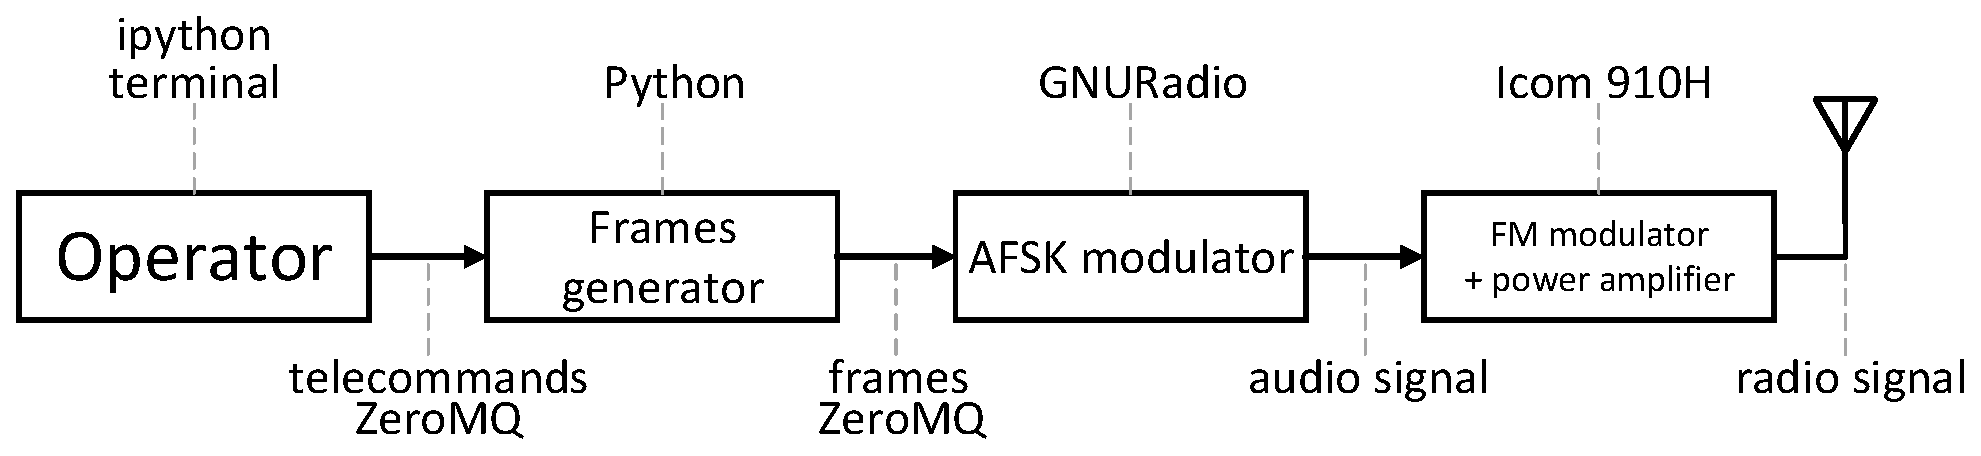
\includegraphics[width=0.6\paperwidth]{img/3/uplink_data_flow.eps}
    \caption{Uplink data flow}
    \label{uplink_data_flow}
\end{figure}

AFSK signal generation GNURadio flowgraph is shown in the figure \ref{uplink_flowgraph}. Audio signal is generated by software Voltage Controlled Oscillator (VCO), and the frequency is controlled by the actual bit value (\SI{1200}{\hertz} or \SI{2200}{\hertz}).

% TODO: uplink_flowgraph


\subsection{Standing Wave Ratio meter}
To check proper antenna connection and ensure long-term monitoring a SWR (Standing Wave Ratio) was installed. This instrument measures ratio of reflected power, thus providing information about antenna impedance matching. In case of antenna break

% TODO: zdjęcie/zrzut z kamerki SWR metera



% ------------------------------------------------------------
% ------------------------- DOWNLINK -------------------------
% ------------------------------------------------------------

\section{Downlink}
Receiving Signals from maximal slant range of about \SI{3000}{\kilo\meter} from a \SI{0.5}{\watt} transmitter requires very high processing gain and low noise factor of the system. System also needs to compensate for Doppler effect and ground interferences.

\subsection{Signal front-end processing}
Radio front-end has two main purposes - to lower the system noise figure (by amplifying the signal with Low Noise Amplifier) and eliminate intermodulation with another signals (filtering). Low Noise Amplifier, installed close to the antenna reduces influence of the long cable to the receiver and reduces the noise added by receiver, reducing total system noise factor. Noise factor is limited by the attenuation between the antenna and Low Noise Amplifier and the Noise Factor of the amplifier itself. However, strong signals in the frequency proximity of the signal can intermodulate in the LNA, resulting in variety of issues: from reduced gain to completely distorted signal.

Narrow-band filter should be installed before the LNA. However, this requires the filter to have the lower loss possible, as the insertion loss of the filter directly affects noise figure of the system. For this purpose, cavity filter was selected. This, narrow band filter (\SI{1}{\MHz}), has very low insertion loss as shown in the measurement chapter. After the filter, Low Noise Amplifier is mounted.

Front-end signal processing is installed as close to the antenna as possible as shown in the figure \ref{elka_skrzynka}.

\begin{figure*}
   \centering
\begin{tabular}{cc}
        \includegraphics[width=0.3\paperwidth]{img/3/elka_view.jpg}
    & 
        \includegraphics[width=0.3\paperwidth]{img/3/elka_skrzynka.jpg}
\end{tabular}
\label{elka_skrzynka}
\caption{PW-Sat2 ground station view and front-end processing.}
\end{figure*}


\subsection{Low noise amplifier design}
A dedicated Low Noise Amplifier was designed. It should eliminate out-of-band signals and amplify the required downlink frequency by at least \SI{20}{\dB}. As the main active component, a high-level Low Noise Amplifier: Mini-Circuits PGA-103+ \cite{lna_pga_datasheet} was used. Additional \SI{433}{\MHz} SAW filter was placed before the amplifier to reduce out of band interferences signals. Bias of the amplifier is created by RF Low Dropout Regulator Texas Instruments TPS7A47 \cite{lna_ldo_datasheet}. Amplifier was designed to support two-stage configuration, but for PW-Sat2 only first stage was populated. Schematic, PCD layout and the picture of the designed board are shown in the figures: \ref{lna_schematic} and \ref{lna_pcb}. The design is open source and all the source files can be found at \cite{lna_github}

\begin{figure}[H]
    \centering
    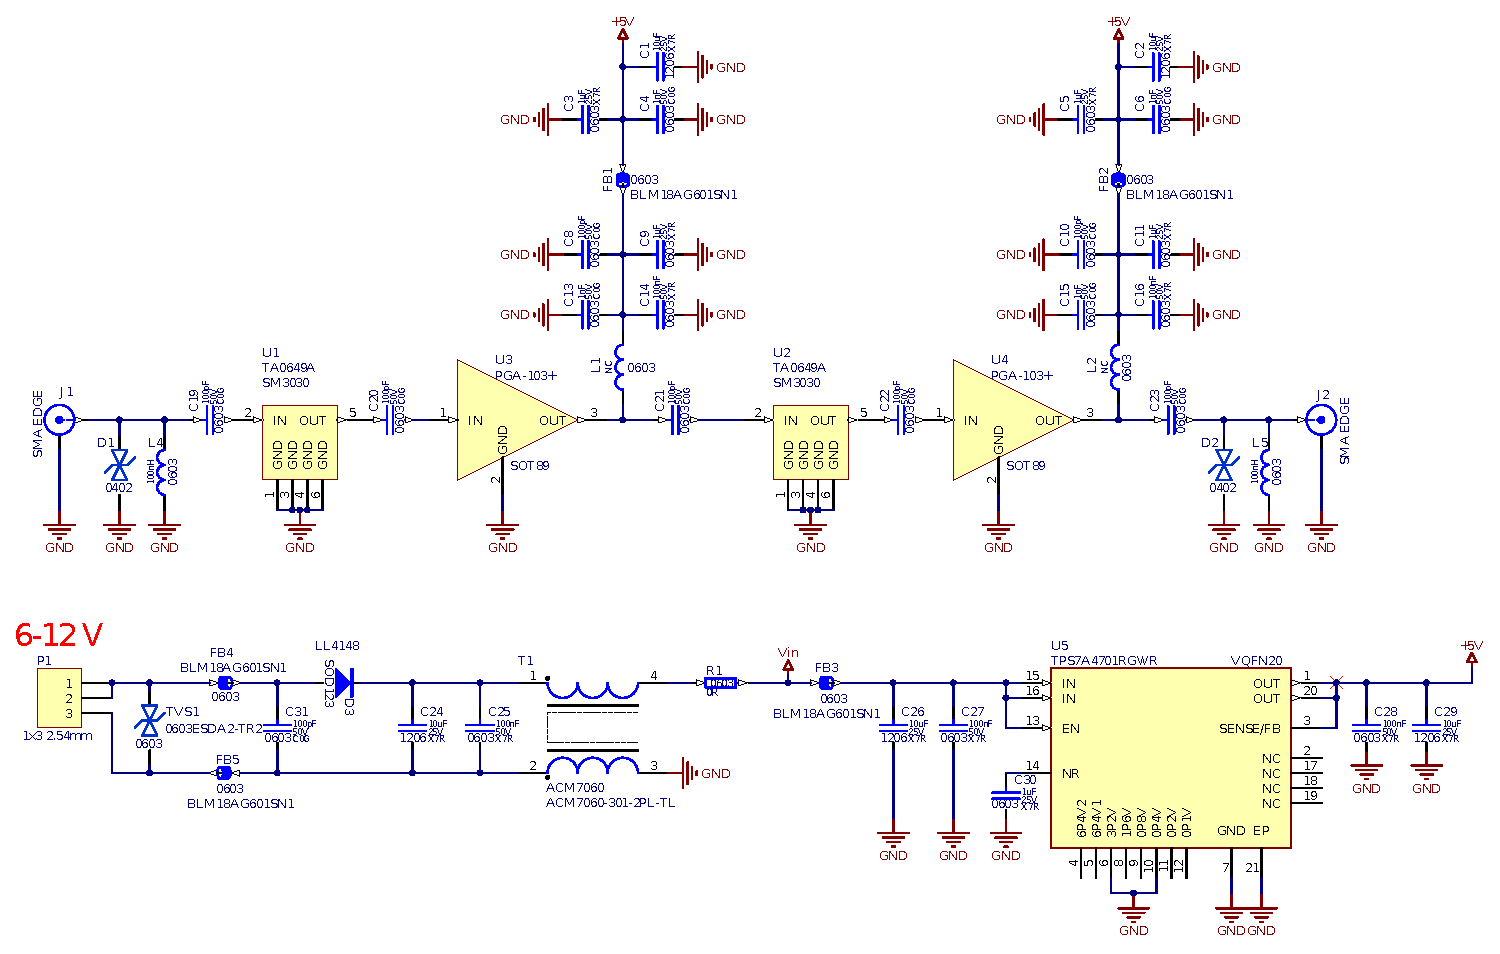
\includegraphics[width=0.8\paperwidth]{img/3/lna_schematic.eps}
    \caption{Low Noise Amplifier Schematic}
    \label{lna_schematic}
\end{figure}

\begin{figure*}
   \centering
\begin{tabular}{cc}
        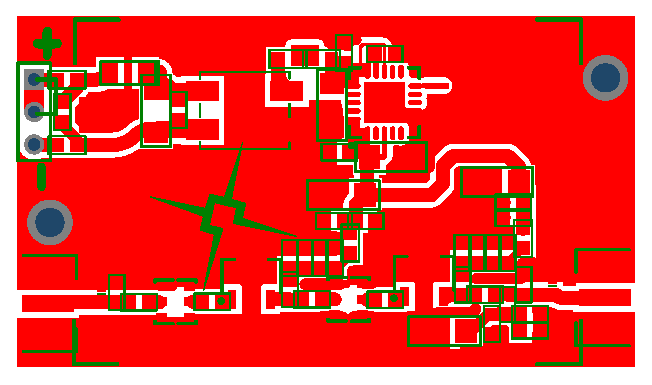
\includegraphics[width=0.4\paperwidth]{img/3/lna_pcb.eps}
    & 
        \includegraphics[width=0.3\paperwidth]{img/3/lna_assembled.jpg}
\end{tabular}
\label{lna_pcb}
\caption{Low Noise Amplifier PCB layout and assembled picture}
\end{figure*}




\subsection{Receiver}
Due to the custom packet format no commercially available integrated circuits were able to correctly receive packets, therefore a custom solution was required for de-modulation and packet recovery.
To receive BPSK signals, the phase recovery is necessary. One of the methods of the synchronous detection is the use of Costas loop \cite{costas_loop}. Most simple solution is to implement full signal chain: Costas loop, bit recovery and packet formatting into software, therefore requiring down-conversion of the signal and data transfer to the PC. 

One of the possible and widely used methods is to use radio amateur transceiver in SSB mode - then radio acts as a multi-stage down-converter, allowing to receive baseband with audio card from PC. However, due to main purpose of transmitting audio signals, there is a lowpass filter for baseband at about \SI{3}{\kHz}. Using SSB mode for receiving PW-Sat2 is possible, however only for \SI{1.2}{\kbps} bitrate.

Another method was to use Software-Defined Radio, performing IQ downconversion and data transmission. The Radio Amateur Satellite Corporation designed an SDR receiver for their mission FUNcube Satellite. After mission success, they released their design and started selling FUNcube dongle shown in the figure \ref{funcube_pic}. Given that is was designed specifically for satellite communication and it was tested using similar CubeSat design, it was selected as the main receiver for PW-Sat2.

\begin{figure}[H]
    \centering
    \includegraphics[width=0.6\paperwidth]{img/2/funcube.jpg}
    \caption{FUNcube Dongle Pro+. Source: \cite{funcube}}
    \label{funcube_pic}
\end{figure}

The receiver  functionalities:
\begin{itemize}
    \item Doppler correction,
    \item IQ data recording,
    \item BPSK demodulation,
    \item bit recovery,
    \item packet formatting,
    \item multiple bitrate simultaneous decoders,
    \item sending data on-line to the operators,
    \item work with different Software-Defined Radios and SSB transceivers
\end{itemize}

The block diagram of the designed system is shown in the figure \ref{demodulator_block_diagram}. All of the signal processing blocks were created using GNUradio framework.

\begin{figure}[H]
    \centering
    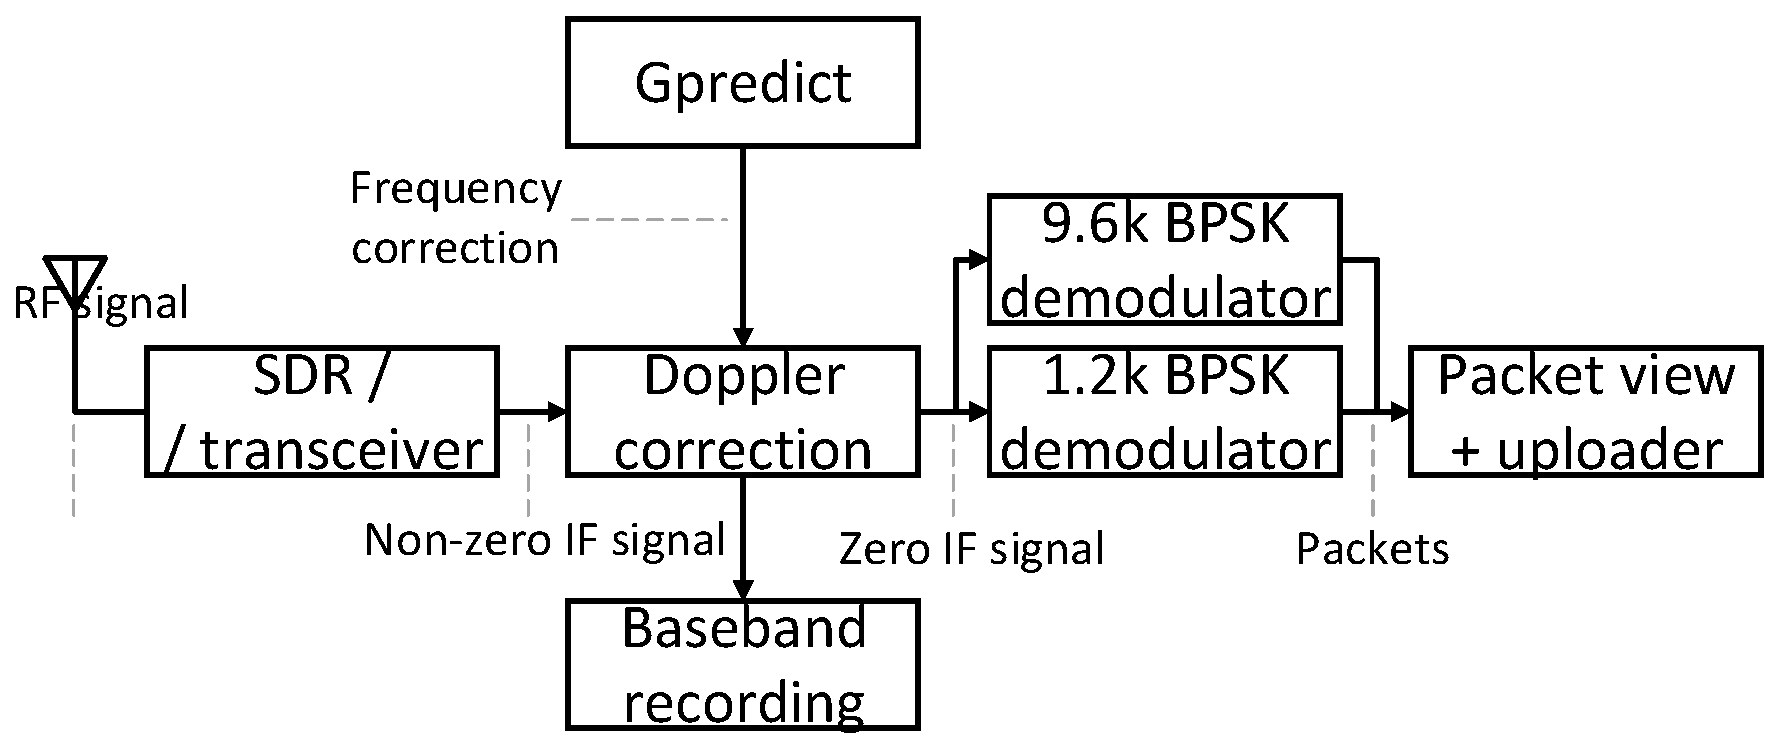
\includegraphics[width=0.6\paperwidth]{img/3/demodulator_block_diagram.eps}
    \caption{Demodulator Block Diagram}
    \label{demodulator_block_diagram}
\end{figure}

First stage, the SDR / transceiver can be any type of Software-Defined radio working with osmocom device drivers, FUNcube SDR or analog SSB radio using audio card. To mitigate the DC-offset and IQ imbalance, the output of this block is on non-zero IF - the frequency of the PW-Sat2 is shifted from the LO frequency. For SSB transceiver, it has to be tuned \SI{2}{\kHz} below the center frequency due to the limited bandwidth of the audio filters. Signal source dialog of the main application is shown in the figure \ref{gs_source_selection}.

\begin{figure}[H]
    \centering
    \includegraphics[width=0.6\paperwidth]{img/3/gs_source_selection.png}
    \caption{Ground station application - signal source selection}
    \label{gs_source_selection}
\end{figure}

Doppler correction is build on quadrature mixer and create zero-IF signal for the next processing blocks. Gpredict calculates required frequency shift and sends it to the block via TCP/IP connection. This updates local VCO frequency for the down-conversion. Latter, the signal is fist-stage filtered and saved to the file for logging purposes. GNUradio block diagram is shown in the figure \ref{gs_doppler_gnuradio}.

\begin{figure}[H]
    \centering
    \includegraphics[width=0.6\paperwidth]{img/3/gs_doppler_gnuradio.png}
    \caption{Doppler correction block GNUradio flowgraph}
    \label{gs_doppler_gnuradio}
\end{figure}

In the system, there are two demodulators (for \SI{1.2}{\kbps} and \SI{9.6}{\kbps} bitrates) operating simulateneously. This allows immediate signal reception during bitrate change by the operator without any manual intervention in the software. Each of them consists of couple of blocks, as shown in the figure \ref{gs_demodulator_diagram}. The demodulator has its own GUI  to show user the status of the demodulation, as shown in the figure \ref{gs_demodulator_gui}.
\begin{itemize}
    \item filtering - low-pass signal with matched Root Raised Cosine filter to eliminate out of band noise,
    \item Costas loop - carrier recovery and phase demodulation,
    \item Symbol synchronisation - recovers bits from the baseband signal, locking a PLL onto the signal,
    \item packet framing - builds a frame from stream of bits,
    \item frame pass to the higher level software.
\end{itemize}

\begin{figure}[H]
    \centering
    \includegraphics[width=0.6\paperwidth]{img/3/gs_demodulator_diagram.png}
    \caption{Ground station demodulator GNUradio flowgraph}
    \label{gs_demodulator_diagram}
\end{figure}

\begin{figure}[H]
    \centering
    \includegraphics[width=0.6\paperwidth]{img/3/gs_demodulator_gui.jpg}
    \caption{Ground station demodulator GUI}
    \label{gs_demodulator_gui}
\end{figure}


After the packet reception, it is shown for the user (as in the figure \ref{gs_frame_view}) and uploaded to the cloud for further analysis by the operations team.

\begin{figure}[H]
    \centering
    \includegraphics[width=0.6\paperwidth]{img/3/gs_frame_view.png}
    \caption{Ground station received frame view}
    \label{gs_frame_view}
\end{figure}